\section{Basic Principles}
The purpose of the fuel cell is to produce an electrical current that can be used to do work like powering a motor or illuminating a light bulb. A chemical reaction inside the fuel cell converts electrochemical energy into electrical energy. A reaction occurs between hydrogen fuel and oxygen or another oxidizing agent creating a DC current. Two electrodes, anode and cathode, allows for a reduction-oxidation process to occur through the catalyst and external electric circuit. 

At the anode, which is the negative electrode, a oxidation process will occur with the following half cell reaction
\begin{equation}
    2H_2 \rightleftharpoons 4H^++ 4e^-
\end{equation}

While at the cathode, which is the positive electrode, the reduction process will occur with the following half cell reaction
\begin{equation}
    O_2 +4H^+ + 4e^- \rightleftharpoons 2H_2O
\end{equation}

This will give us a overall reaction as following
\begin{equation}
    2H_2 + O_2 \rightleftharpoons 2H_2O
\end{equation}


Pressurized hydrogen $(H_2)$ will enter at the anode where it will come in contact with the catalyst causing the $H_2$ molecule to split into two $H^+$ ions and two electrons. At the opposite side, oxygen gas $(O_2)$ will enter at the cathode and form two oxygen atoms with strong negative charges. This negative charge will attract the $H^+$ ions to pass through the membrane, while the electrons are blocked from passing through the membrane and forced through an external circuit. On the other side the $H^+$ ions will recombine with an oxygen atom and two electrons from the external circuit to create a water molecules $(H_2O)$.


Since the fuel cell creates electricity from a chemical reaction, rather than combustion, it will not be a subject to thermodynamic laws like "Carnot Limit" and will be more efficient in transforming energy from fuels to usable electrical energy. To further increase the efficiency of the fuel cell, the waste heat can be harnessed. However activation energy needs to be supplied to cross the thermodynamic barrier.

To cross this thermodynamic barrier a  catalyst can be applied to the electrodes and the membrane to increase the kinetics of the reaction which will determine how fast the reactions occurs. We can also increase the surface area of the electrodes, as well as raise the temperature. 

\begin{figure}[ht]
    \centering
    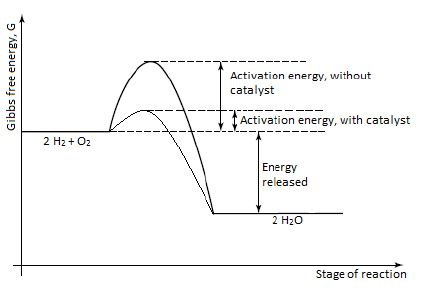
\includegraphics[width=0.9\textwidth]{DIV./Bilder/activation.jpg}
    \caption{Activation energy diagram}
    \label{fig:Activation}
\end{figure}

The driving force of these chemical reactions is the Gibbs free energy and change in Gibbs free energy lets us calculate the ideal no loss voltage for a single cell to 1.23 V with the following equation
\begin{equation}
    \Delta G = zFE^0
\end{equation}

Where
\begin{center}
    $\Delta$G = Change in Gibbs free energy under standard conditions [$J/Mol$] \\
    z = Number of electrons [-] \\
    F = Faradays constant [$C/Mol$] \\
    $E^0$ = EMF under standard conditions [$V$]
\end{center}

In reality a fuel cell will have lower voltage because of losses. Some losses are caused by fuel crossover, internal current losses, ohmic losses, and mass transport or concentration losses. The Cell voltage output is given by the following
\begin{equation}
    V_{cell} = E_{ocv} - \Delta V_{activasion} - \Delta V_{ohmic} - \Delta V_{mass}
\end{equation}

$E_{ocv}$ is given by the thermodynamic EMF

\begin{equation}
    E_{ocv} = - \frac{\Delta G}{zF}
\end{equation}


\begin{figure}[ht]
    \centering
    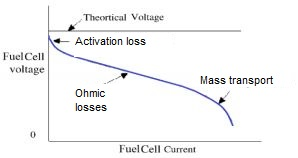
\includegraphics[width=0.9\textwidth]{DIV./Bilder/Assembly/losses.jpg}
    \caption{Fuel cell current-voltage characteristic}
    \label{fig:Fuel cell current-voltage characteristic}
\end{figure}

The efficiency of the PEMFC is calculated using the following equation
\begin{equation}
    \eta =  \frac{E_1}{E^0}
\end{equation}

Where
\begin{center}
$\eta$ = the efficiency of the fuel cell \\
$E_1$ = Measured fuel cell voltage \\
$E^0$ = No loss voltage    
\end{center}

Another challenge with the PEMFC is water balance. In each cell water is being formed and depending on operating conditions and the load, the fuel cell can both be flooded and dried out. If the fuel cell is flooded it can prevent reactant diffusion to the catalyst by flooding the electrodes. A dried-out fuel cell will decrease the electrolytes proton conductivity, which will increase the cell resistance and decrease the efficiency of the fuel cell. It is important that the membrane has just the right moisture level without flooding or drying it out to get the best possible efficiency.

.....Gas diffusion, for å spre gassen mest mulig slik at man får flest mulig reaksjoner.....

\section{Components}

\begin{figure}[h]
    \centering
    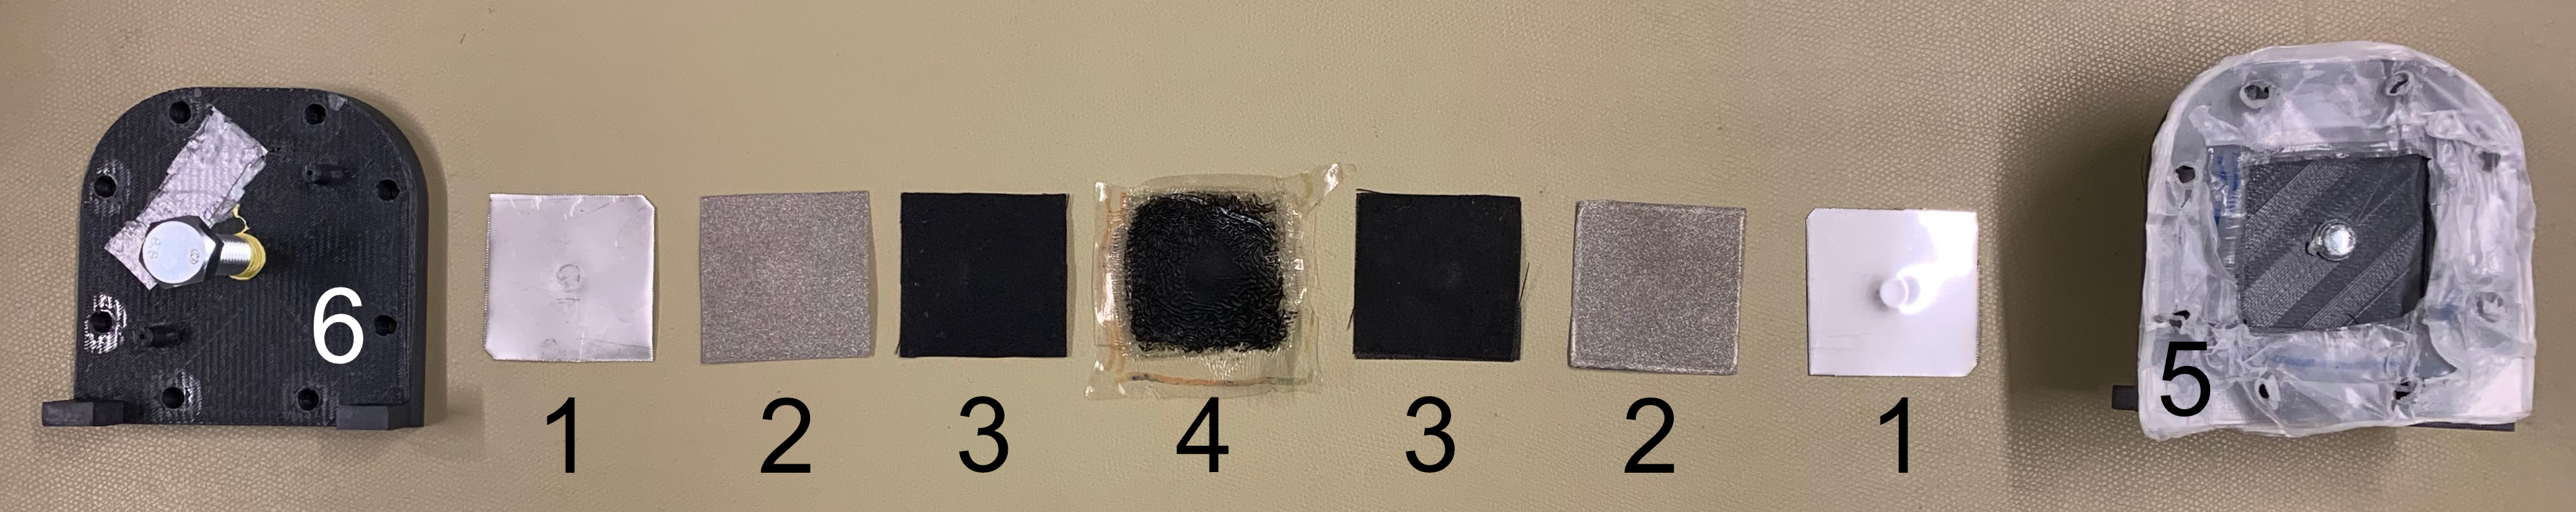
\includegraphics[width=\textwidth]{DIV./Bilder/layout.jpg}
    \caption{Components in PEM fuel cell}
    \label{fig:Components}
\end{figure}

\subsection{Anode and cathode}
Hydrogen will enter at the negative electrode of the PEMFC called the anode. The job of the anode is to conduct electrons that are freed from the hydrogen molecules to be used in an external circuit. Our anode is a carbon paper with a thin layer of catalyst on the side facing the membrane.

Oxygen will enter at the positive electrode of the PEMFC called the cathode. Just as our anode, the cathode is a carbon paper with a thin layer of catalyst on the side facing the membrane. The job of the cathode is to conduct electrons back from the external circuit to the catalyst, here they will recombine with $H^+$ ions and oxygen to form water. The anode and cathode can be seen on figure \ref{fig:Components}

\begin{figure}[h]
    \centering
    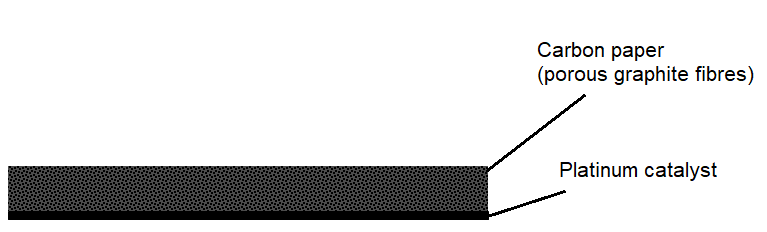
\includegraphics[width=0.6\textwidth]{DIV./Bilder/carbonpaper.png}
    \caption{Electrodes - Carbon paper}
    \label{fig:Electrodes}
\end{figure}

\subsection{Electrolyte}
Ath the heart of the fuel cell sits an electrolyte  and in a PEMFC this is a proton exchange membrane. This membrane allows $H^+$ ions to pass through unhindered while electrons and other substances are blocked from passing through. The membrane is made up by a specially treated material, so that it only conducts positively charged ions. The electrolyte in a  PEMFC is usually is a thin transparent proton exchange membrane called Membrane Electrolyte Nafion (MEA) with a thickness of about \( 50\ \mu \)m


\begin{figure}[h]
    \centering
    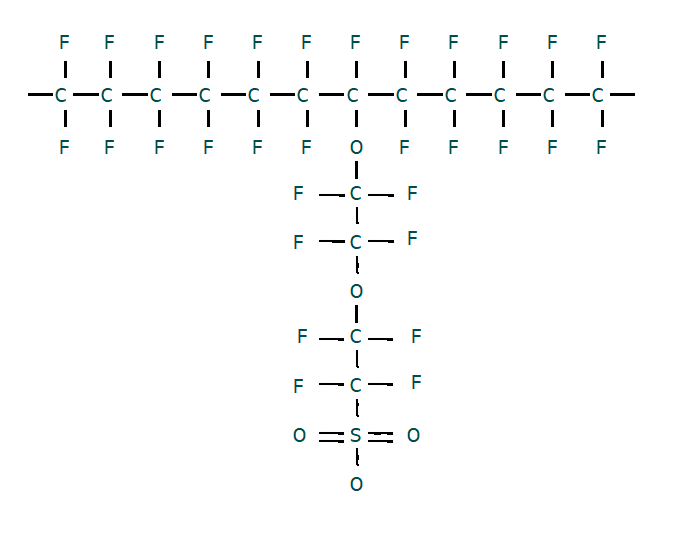
\includegraphics[width=0.7\textwidth]{DIV./Bilder/polymersheet.png}
    \caption{Sulphonated flourethylene Nafion \cite{PemLectue}}
    \label{fig:Nafion}
\end{figure}

\subsection{Catalyst}
The catalyst in our PEMFC is a mix of carbon-platinum and isopropyl alcohol (IPA) painted onto both sides of our electrolyte and also onto both of the carbon electrodes.

This is made up of a special material that facilitates the reaction of oxygen and hydrogen. It is most commonly made up by a very thin coat of platinum nanoparticles onto carbon paper or a piece of cloth. To expose the hydrogen and oxygen as much as possible to the platinum the catalyst will be rough and porous. 

\begin{wrapfigure}{r}{0.5\textwidth}
  \begin{center}
    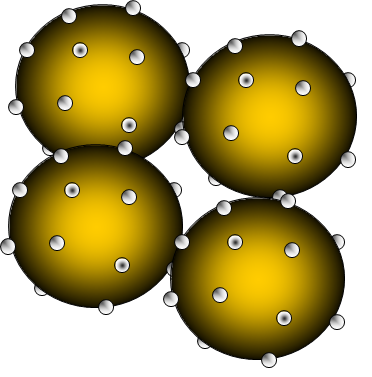
\includegraphics[width=0.3\textwidth]{DIV./Bilder/Catalyst.png}
  \end{center}
  \caption{Small platinum particles on carbon particles \cite{PemLectue}}
\end{wrapfigure}